% Define a section
\section{Názov kapitoly}
Lorem ipsum dolor sit amet, consectetur adipiscing elit. Integer eu lacus leo. Nulla egestas purus non dignissim tincidunt. In sit amet tellus bibendum, lobortis magna ut, sodales mi. Etiam vel eros efficitur purus ultrices vulputate et quis justo. Nunc ultrices tellus a dui mattis, eget laoreet arcu tempor. Donec vestibulum, magna ac fringilla lacinia, libero risus fringilla arcu, nec consectetur nibh justo vel sem. Quisque gravida sit amet elit ut aliquam.....

% Define a subsection
\subsection{Názov podkapitoly}
Lorem ipsum dolor sit amet, consectetur adipiscing elit. Integer eu lacus leo. Nulla egestas purus non dignissim tincidunt. 
\begin{itemize}
    \item Položka zoznamu
    \item Položka zoznamu
\end{itemize}
\hfill
\begin{enumerate}
    \item Položka číslovaného zoznamu
    \item Položka číslovaného zoznamu
\end{enumerate}

% Add a figure
\begin{figure}[h]
    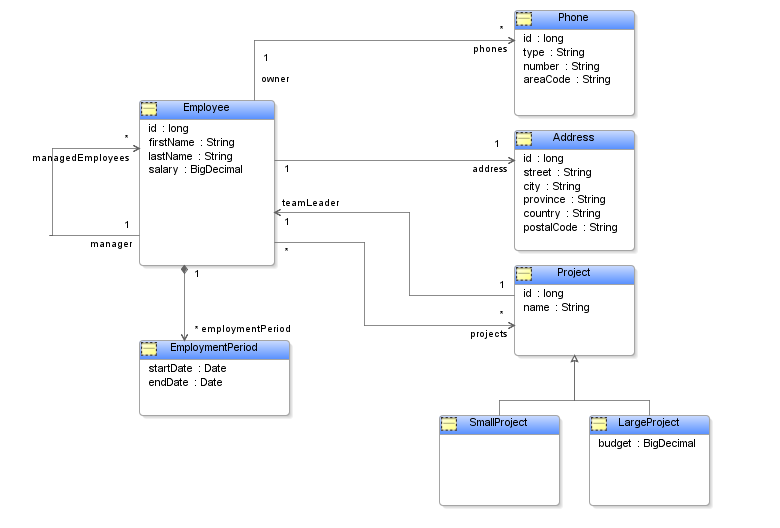
\includegraphics{examples/images/employee-model.png}
    \caption{UML diagram zamestnanca}
    \label{fig:example1}
\end{figure}

% Add citations
\newpage
\noindent
Odkazy na použitú literatúru \parencite{luptak2016thesis} alebo \textcite{borgman2003from}.\footnote{V prípade nejasností alebo pre lepšie pochopenie niektorých pojmov jazyka boli ďalej využívané aj zdroje \parencite{lynch2005where} a \parencite{luptak2016thesis}}
\\Pre citácie používajte normu STN ISO 690, môžete citovať aj v tvare [1], [2],… vtedy v zozname literatúry neuvádzate zdroje abecedne, ale ich uvádzate podľa poradia výskytu v texte. 

% Define a subsubsection
\subsection{Môžete vložiť novú podkapitolu}
\subsubsection{Taktiež aj na úrovni 3}

% Add a table
\begin{table}[!h]
    \centering
    \caption{Názov tabuľky}
    {\color{red} \textbf{Pánsky dres - strih Classic}}\\
    \vspace{1em}
    \rowcolors{2}{white}{gray!30}  
    \begin{tabular}{cccc}  
        \textbf{dres - veľkosť} & \textbf{obvod hrudník} & \textbf{obvod pás (guma)} & \textbf{dĺžka zadného dielu (od krku)} \\
        XS & 96 & 72-80 & 69 \\
        S & 100 & 76-84 & 70 \\
        M & 104 & 80-80 & 71 \\
        L & 108 & 84-96 & 72 \\
        XL & 112 & 88-100 & 73 \\
        XXL & 116 & 92-104 & 75 \\
        XXXL & 120 & 96-108 & 77 \\
    \end{tabular}
    \label{tab:example}
\end{table}

% Add a code block
\begin{lstlisting}[language=Python, caption={Príklad kódu v Pythone}, label={lst:python-example}]    
def hello_world():
    print("Hello, world!")
        
# Example class
class Person:
    def __init__(self, name):
        self.name = name
    
    def greet(self):
        return f"Hello, my name is {self.name}"

# Create instance
person = Person("Alfred")
print(person.greet())
\end{lstlisting}